% options:
% thesis=B bachelor's thesis
% thesis=M master's thesis
% czech thesis in Czech language
% slovak thesis in Slovak language
% english thesis in English language
% hidelinks remove colour boxes around hyperlinks

\documentclass[thesis=B,czech]{FITthesis}[2012/06/26]

\usepackage[utf8]{inputenc} % LaTeX source encoded as UTF-8

\usepackage{graphicx} %graphics files inclusion
% \usepackage{amsmath} %advanced maths
% \usepackage{amssymb} %additional math symbols

\usepackage{dirtree} %directory tree visualisation 
\RequirePackage{pdfpages}
\usepackage{float}
\usepackage[all]{nowidow}

% % list of acronyms
% \usepackage[acronym,nonumberlist,toc,numberedsection=autolabel]{glossaries}
% \iflanguage{czech}{\renewcommand*{\acronymname}{Seznam pou{\v z}it{\' y}ch zkratek}}{}
% \makeglossaries

\newcommand{\tg}{\mathop{\mathrm{tg}}} %cesky tangens
\newcommand{\cotg}{\mathop{\mathrm{cotg}}} %cesky cotangens

% % % % % % % % % % % % % % % % % % % % % % % % % % % % % % 
% ODTUD DAL VSE ZMENTE
% % % % % % % % % % % % % % % % % % % % % % % % % % % % % % 

\department{Katedra Softwarového inženýrství}
\title{Webový frontend informačního systému}
\authorGN{Jakub} %(křestní) jméno (jména) autora
\authorFN{Doležal} %příjmení autora
\authorWithDegrees{Jakub Doležal} %jméno autora včetně současných akademických titulů
\author{Jakub Doležal} %jméno autora bez akademických titulů
\supervisor{Ing. Jiří Chludil}
\acknowledgements{Doplňte, máte-li komu a za co děkovat. V~opačném případě úplně odstraňte tento příkaz.}
\abstractCS{Cílem této práce je návrh, implementace a otestování webového frontendu informačního systému pro firmu MAHALUX s.r.o.
	
	Na základě požadavků zadavatele je tento webový frontend implementovaný pomocí frameworku ReactJS v jazyce JavaScript. Serverová část aplikace je implementována v jazyce PHP s využitím frameworku Nette.
	
	Tento informační systém napomáhá k rychlému, hromadnému a bezchybnému zadávání dat. Zefektivňuje a centralizuje evidenci dat prováděnou zaměstnanci MAHALUX s.r.o.
	
	V uživatelské příručce jsou popsány složitější případy užití tohoto frontendu.
}
\abstractEN{Sem doplňte ekvivalent abstraktu Vaší práce v~angličtině.}
\placeForDeclarationOfAuthenticity{V~Praze}
\declarationOfAuthenticityOption{4} %volba Prohlášení (číslo 1-6)
\keywordsCS{webový frontend, informační systém, návrh, implementace, testování, hromadné zadávání dat, ReactJS, PHP, Nette framework}
\keywordsEN{web frontend, information system, design, implemtation, test, bulk data input, ReactJS, PHP, Nette framework}
% \website{http://site.example/thesis} %volitelná URL práce, objeví se v tiráži - úplně odstraňte, nemáte-li URL práce


\begin{document}

% \newacronym{CVUT}{{\v C}VUT}{{\v C}esk{\' e} vysok{\' e} u{\v c}en{\' i} technick{\' e} v Praze}
% \newacronym{FIT}{FIT}{Fakulta informa{\v c}n{\' i}ch technologi{\' i}}

\begin{introduction}
	MAHALUX s.r.o. je mladá expandující firma zabývající vývojem, výrobou a prodejem elektronický zařízení. I přesto že firma existuje poměrně krátce, již expeduje po celém světě. To přináší velké nároky na evidenci rozličných dat o adresách, bankovních spojeních a dalších informacích o zákaznících. Proto se firma MAHALUX s.r.o. rozhodla pro zavedení informačního systému s webovým frontendem, který přinese potřebné centralizované ukládání dat a pohodlný přístup k těmto datům.
	
	V práci se zabývám analýzou, návrhem, implementací a testováním webového informačního systému.
	Úkolem úvodní části práce je sběr funkčních a nefunkčních požadavků zadavatele. Dále také analýza složitějších případů užití.
	Následuje návrh struktury systému, návrh komponetového prototypu a uživatelského rozhraní v knihovně ReactJS. Navazovat bude samotná implementace a na závěr testování.
\end{introduction}

\chapter{Cíl práce}
	Cílem rešeršní části práce je analýza požadavků zákazníka a analýza složitějších případů užití. Dále prozkoumání existujících řešení webových frontendů pro získání přehledu o best practicies. Mimo jiné se zaměřím na možnosti continuous integration a continuous deployment a jejich využití pro tento projekt. A v neposlední řadě provedu rešerši databázových enginů. Především porovnám open-source řešení MySQL a PostrgeSQL.
	
	Cílem praktické části práce je návrh, implementace a otestování webového frontendu tohoto informačního systému. Hlavní důraz bude kladen dynamičnost uživatelského rozhraní. To by mělo uživateli napomáhat k co nejrychlejšímu a pokud možno bezchybnému vkládání dat. K tomu budou využity šablony, které si uživatel nadefinuje společně s daty a ty následně ze šablony vloží do konkrétního formuláře. Dále by měla být zajištěna přehledná reprezentace větších záznamů a hromadné úpravy. Systém bude komponentový pro zaručení možnosti jednoduchého rozšíření systému.
	
\chapter{Analýza a návrh}

\section{Specifikace systémových požadavků}

	Na základě komunikace s firmou MAHALUX s.r.o. byly stanoveny následující systémové požadavky.
	
\subsection{Funkční požadavky}

\begin{enumerate}
	\item Agenda faktur a fakturovaných katalogových položek(fakturováno může být několik katalogových položek v počtu jeden a více)
	\begin{itemize}
		\item Přehled evidence vydaných faktur a fakturovaných položek a pro jednotlivé faktury:
		\begin{itemize}
			\item vytvoření nové faktury
			\item editace faktury
			\item smazání faktury 
			\item tisk faktury.
		\end{itemize}
		\item Formulář pro vytvoření a úpravu 1 nebo více faktur na základě jedné nebo více objednávek - zajistit předvyplnění fakturačních položek na základě položek v objednávce či objednávkách.
		\item Přehled přijatých faktur a pro jednotlivé faktury:
		\begin{itemize}
			\item Uložení přijaté faktury včetně souborů,
			\item Změna stavu faktury (přijatá, částečně uhrazená, uhrazená),
			\item smazání faktury a
			\item tisk faktury.
		\end{itemize}
	\end{itemize}	
	\item Evidence nabízených produktů
		\begin{itemize}
			\item Vyhledání, přidání, úprava a smazání nabízeného produktu
		\end{itemize}
	\newpage
	\item Agenda firemního skladu
		\begin{itemize}
			\item evidovat skladové pohyby u jednotlivých produktů
			\item přehled položek ve skladu
			\item editace položek skladu
		\end{itemize}
	\item Agenda objednávek - přehled evidovaných objednávek a pro jednotlivé objednávky:
	\begin{itemize}
		\item vložení nové objednávky
		\item editace objednávky
		\item smazání objednávky
		\item vytvoření faktur na základě jedné nebo více objednávek
		\item evidencí trackingu po expedování
	\end{itemize}
	\item Formulář pro přípravu expedice položek objednávky
	\begin{itemize}
		\item Formulář zobrazí objedané množství produktů a množství produktů na skladě. 
		\item Přednastaví množství k odeslání podle toho zda je možné objednávku kompletně vybavit či ne.
		\item Potvrzením vložení do expedice při nenulovém množství k odeslání dojde k vytvoření záznamů o balíčcích a jejich zařazení do následující expedice.
	\end{itemize}
	\item Agenda dodávek
	\begin{itemize}
		\item Přehled objednaných dodávek včetně trackingu.
		\item Formulář pro vložení nové dodávky včetně trackingu
		\item Editace dodávky v případě špatně nebo nekompletně dodané dodávky
		\item Označení dodávky jako dodané způsobí automatické naskladnění
	\end{itemize}
	\item Agenda kontaktů
	\begin{itemize}
		\item Na základě příznaku evidovat dodavatele a odběratele
		\item Evidovaní budou dodavatelé - právnické osoby
		\item Evidence odběratelů
		\begin{itemize}
			\item Právnické osoby
			\item Fyzické osoby
		\end{itemize}
	\end{itemize}
	\newpage
	\item Hromadné úpravy
	\begin{itemize}
		\item Více záznamů lze editovat jako jeden. 
		\item Pokud jsou původní hodnoty stejné, zobrazí se k úpravě stejně jako by se editoval jeden záznam. 
		\item Pokud jsou původní hodnoty rozdílné, namísto pole k editaci se zobrazí tlačítko pro výběr jedné společné hodnoty (ideálně histogram), kterou lze potom opět editovat jako jednu hodnotu. Pokud se hodnota neupraví, zůstávají původní hodnoty.
	\end{itemize}
	\item Vyplňování formuláře šablonou
	\begin{itemize}
		\item Uživatel si nadefinuje šablonu s konkrétními daty v konkrétních polích a šablonu uloží. 
		\item Při další vyplňování téhož formuláře bude moci vybrat uloženou šablonu a ta mu formulář vyplní uloženými daty. 
		\item Uživatel bude dále moci data upravit a případně šablonu upravit či uložit novou.
	\end{itemize}
	\item Management uživatelů
	\begin{itemize}
		\item O každém uživateli evidovat loginID, username, skutečné jméno, heslo.
		\item Každý uživatel má nějaké oprávnění. Oprávnění mohou být admin, expeditér.
		\item Založení uživatele.
		\item Upravení uživatele.
		\item Deaktivace uživatele.
		\item Přehled uživatelů.
		\item Administrátor bude moci vygenerovat uživateli nové heslo při zapomenutí hesla.
	\end{itemize}
	\item Evidence úprav dat (kdo data upravil a kdy)
	\begin{itemize}
		\item Pro každý záznam ve všech tabulkách bude evidováno kdo a kdy řádek vytvořil, upravil a smazal(technika soft delete)
		\item To kým byla data upravena bude zaznamenáno z loginu uživatele.	
	\end{itemize}
	\item Vytvořit API pro manipulaci se všemi tabulkami
\end{enumerate}

\subsection{Nefunkční požadavky}
\begin{enumerate}
	\item Odezvy v reálném čase (typicky maximálně 100 ms na 1000000 záznamů, u větších tabulek základní stránkování s použitím indexů)
	\item Konzistence dat - na úrovni DB transakcí (server splňuje ACID)
	\item Dynamicky reagující formuláře
	\begin{itemize}
		\item Určená pole formuláře reagují na změnu v jiném poli. Například při výběru/zadání hodnoty v kolonce země se v návaznosti na to upraví nabídka v kolonce stát. 
		\item Pokud je pro dané pole možné vyplnit pouze jednou hodnotu, bude tato hodnota automaticky doplněna.
	\end{itemize}
	\item[4.NF] Našeptávač
	\begin{itemize}
		\item Při zapisování údaje do určené kolonky systém automaticky napovídá zbylou část textu.
		\item Je potřeba, aby mohl našeptávat z více sloupců, včetně cizích. 
		\item Našeptávač se bude využívat při odkazování na informace z jiné tabulky. Například při výběru položky z objednávky, našeptávač našeptává počet kusů z tabulky položky objednávky a název položky z tabulky číselníku. Vždy budou určeny konkrétní sloupce z odkazované tabulky.
	\end{itemize}
	\item Editace položek přehledů v pop-up okně
\end{enumerate}

\subsection{Požadavky na rozhraní}
\begin{enumerate}
	\item Integrace do MySQL databáze a souborového systému pro upload příloh.
	\item Přívětivé uživatelské rozhraní v ReactJS napomáhající uživateli práci odvést rychle a bezchybně.
\end{enumerate}

\section{Doménový model}
	Doménový model popisuje entity a vazby mezi nimi v doméně e-shopu firmy MAHALUX s.r.o.
	
\begin{figure}[H]
	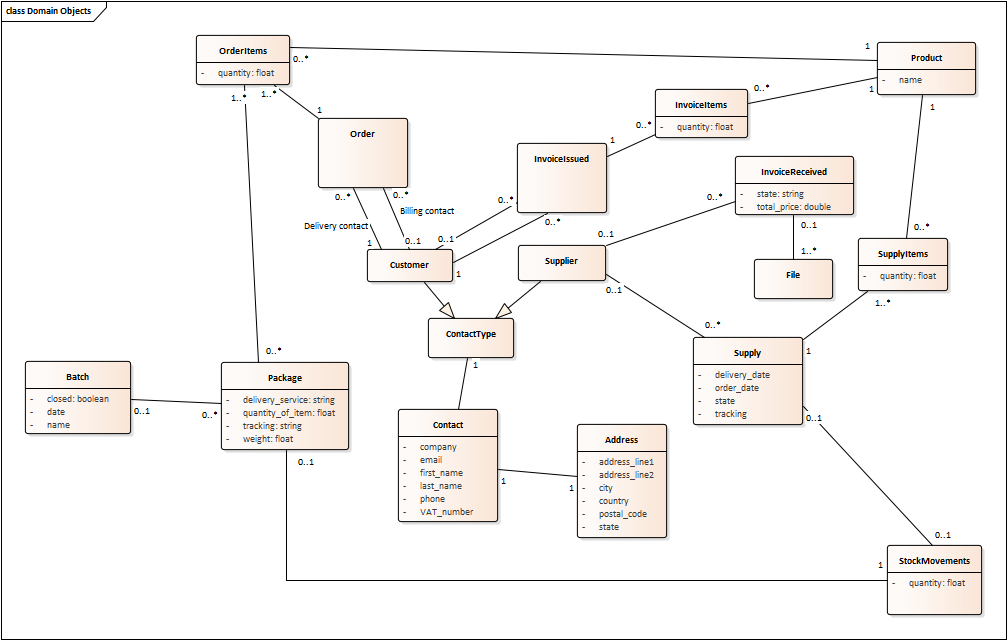
\includegraphics[height=\textwidth, angle=90]{domain_model.png}
	\caption{Doménový model}\label{domain_model}
\end{figure}

\section{E-R model}
E-R model popisuje entity se všemi vlastnostmi a vazby mezi nimi.

\begin{figure}[H]
	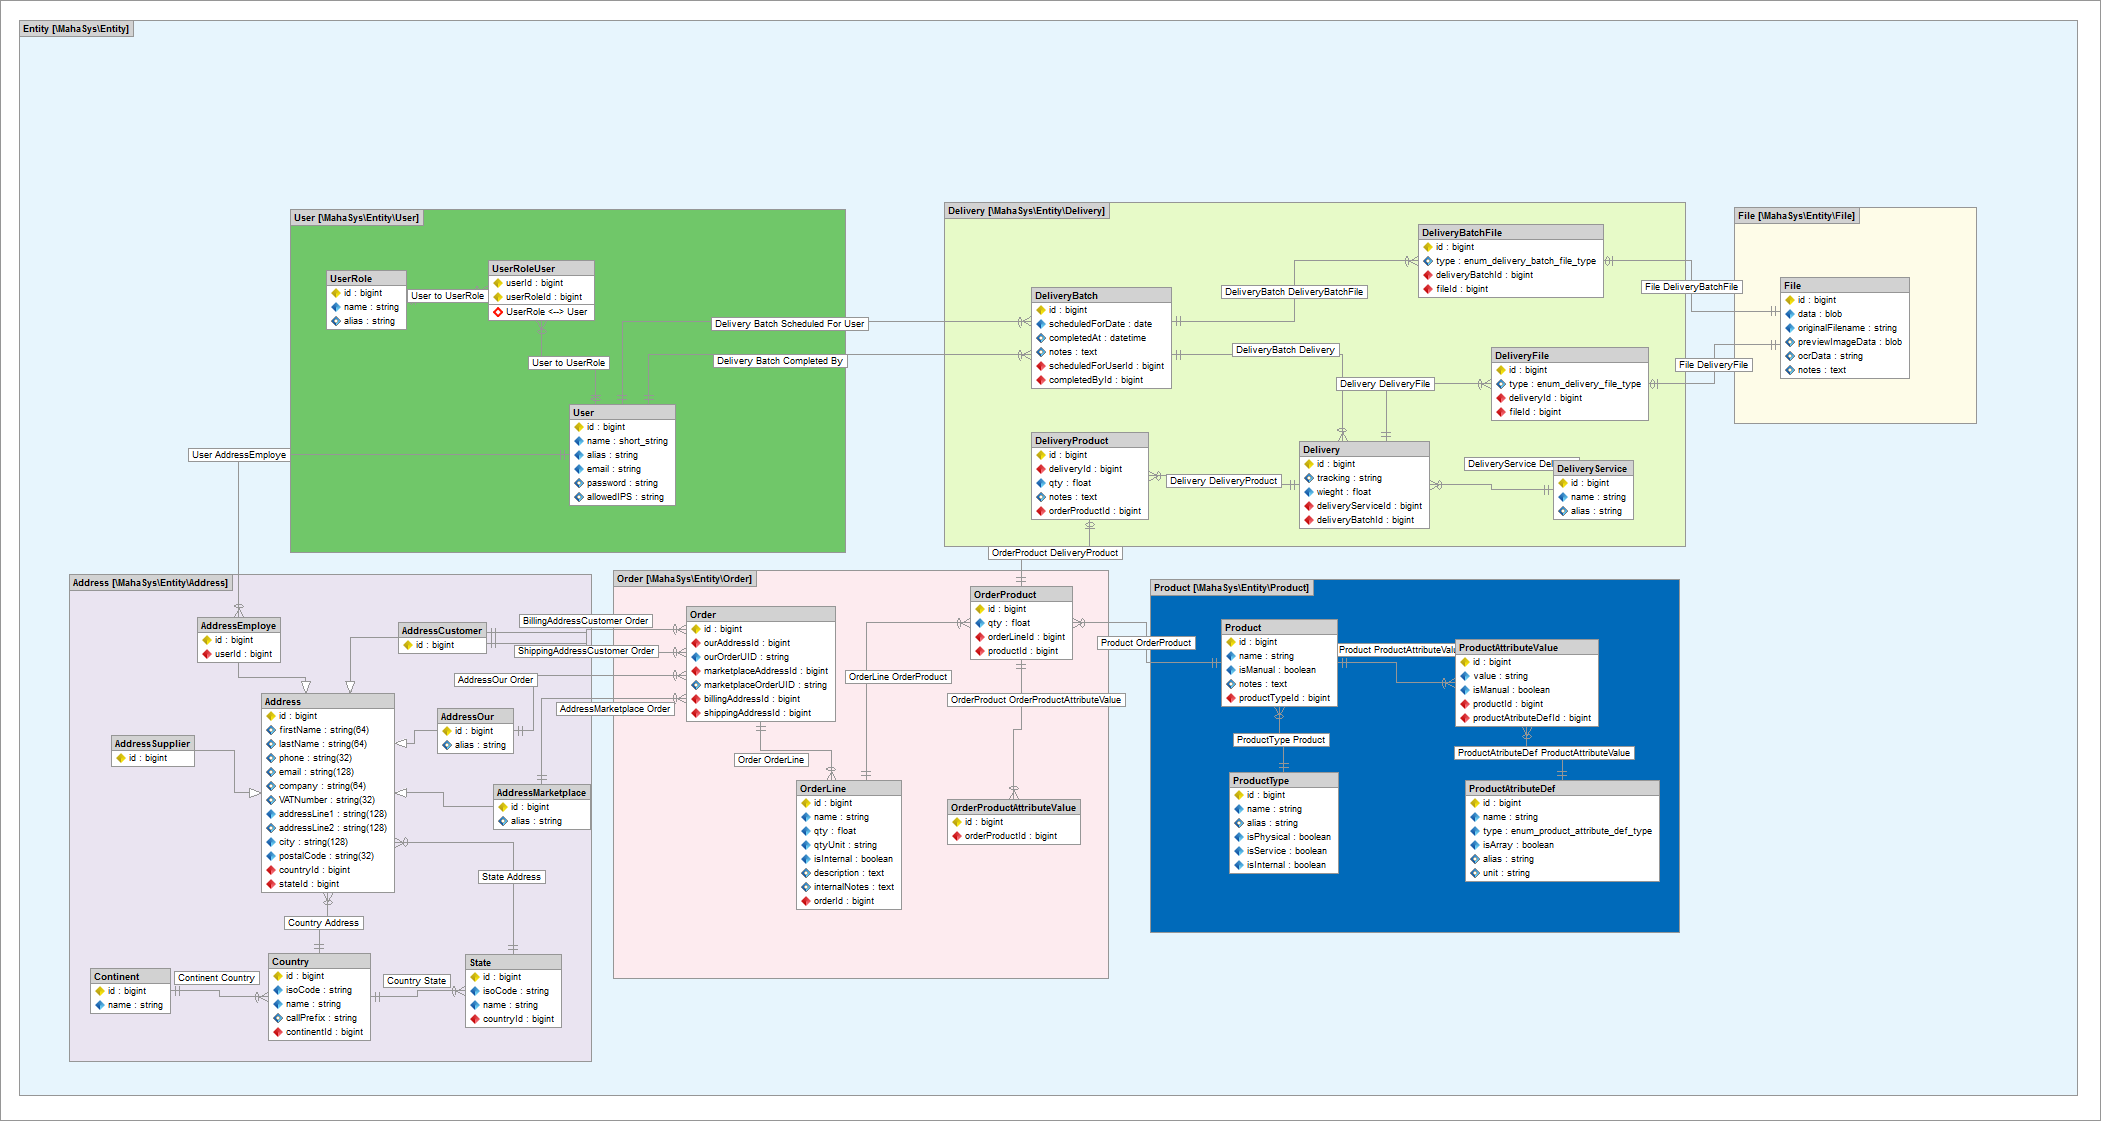
\includegraphics[width=500pt, height=\textwidth, angle=90]{mahasys_ermodel.png}
	\caption{E-R model}\label{er_model}
\end{figure}

\section{Výběr modelovacího nástroje s ohledem na možnosti generování zdrojového kódu modelu}
	Nástroj s možností generování modelu může velice pomoci při vývoji. V první řadě je potřeba pro vizualizaci problémové domény. Za druhé lze některé takové nástroje použít pro generování zdrojového kódu modelu nebo pro vytvoření databázových DDL skriptů. Pro potřeby systému jsem se zaobíral především možností generovat gettery a settery a možností definice ORM notace pro Doctrine 2.

\subsection{Enterprise Architect}
	Enterprise Architect je poměrně robustní UML nástroj pro modelování celého vývojového cyklu softwaru. Pokrývá vše od sběru požadavků, modelování business procesů, architektury, domény až po class diagramy, či databázové modely. Dále umožňuje generování zdrojových kódů modelu včetně getter a setterů pro jazyky Java, C++, C\#, Python, PHP, aj., které provádí na základě modifikovatelných šablon. Tyto šablony využívají vlastní jazyk nazýváný Transformation Template language. Enterprise Architect také nabízí generování DDL skriptů pro mnoho databázových enginů jako jsou Oracle, MySql, SQL Server a další.

\subsection{Skipper}
	Skipper je E-R modelář zaměřený na programovací jazyk PHP. Umožňuje generovat zdrojový kód modelu s ohledem na použitý MVC framework a také dle zvolené ORM knihovny. Tím nepřímo přinese databázové DDL skripty. U Doctrine toto zajistí schema-tool, nástroj pro manipulaci s databázovým modelem používaný z příkazové řádky. Podporuje ORM knihovny Doctrine, Doctrine 2, Propel a CakePHP.
	
\subsection{Srovnání}
	Skipper je určitě lépe připravený na ORM, to EA neřeší vůbec. Naopak v Enterprise Architectu lze generování pomocí doupravit a plně nakonfigurovat. To může být velmi užitečné například při použití traitu společného pro všechny třídy reprezentující databázové entity. Jednoduše se použití traitu vloží do šablony. Skipper toto neumožňuje a přidání je nutné dělat ručně. Nicméně vyladění šablon Entreprise Architectu pro generování zdrojového kódu by stálo hodně úsilí s nejistým výsledkem. Proto jsem se rozhodl pro využití Skipperu i přes jeho slabší konfigurovatelnost.	

\chapter{Realizace}

\section{praktická část}

\begin{conclusion}
	%sem napište závěr Vaší práce
	%shrnutí míry uspěšnosti realizace cíle a jak jsme toho dosáhli
	%výhled do budoucna - možné rozšíření výsledku práce
	Cílem práce byl návrh, implementace a otestování webového frontendu informačního systému.
	
	Aplikace byla nasazena. Splňuje požadavky zadané zadavatelem. Napomáhá rychle a bezchybně evidovat data. Je napojena na interní databázi kde ukládá zadávaná data.
\end{conclusion}

\bibliographystyle{csn690}
\bibliography{mybibliographyfile}

\appendix

\chapter{Seznam použitých zkratek}
% \printglossaries
\begin{description}
	\item[GUI] Graphical user interface
	\item[DDL] Data definition language
	\item[UML] Unified Modeling language
	\item[ORM] Object relation mapping
	\item[MVC] Model-view-controller
\end{description}


% % % % % % % % % % % % % % % % % % % % % % % % % % % % 
% % Tuto kapitolu z výsledné práce ODSTRAŇTE.
% % % % % % % % % % % % % % % % % % % % % % % % % % % % 
% 
% \chapter{Návod k~použití této šablony}
% 
% Tento dokument slouží jako základ pro napsání závěrečné práce na Fakultě informačních technologií ČVUT v~Praze.
% 
% \section{Výběr základu}
% 
% Vyberte si šablonu podle druhu práce (bakalářská, diplomová), jazyka (čeština, angličtina) a kódování (ASCII, \mbox{UTF-8}, \mbox{ISO-8859-2} neboli latin2 a nebo \mbox{Windows-1250}). 
% 
% V~české variantě naleznete šablony v~souborech pojmenovaných ve formátu práce\_kódování.tex. Typ může být:
% \begin{description}
% 	\item[BP] bakalářská práce,
% 	\item[DP] diplomová (magisterská) práce.
% \end{description}
% Kódování, ve kterém chcete psát, může být:
% \begin{description}
% 	\item[UTF-8] kódování Unicode,
% 	\item[ISO-8859-2] latin2,
% 	\item[Windows-1250] znaková sada 1250 Windows.
% \end{description}
% V~případě nejistoty ohledně kódování doporučujeme následující postup:
% \begin{enumerate}
% 	\item Otevřete šablony pro kódování UTF-8 v~editoru prostého textu, který chcete pro psaní práce použít -- pokud můžete texty s~diakritikou normálně přečíst, použijte tuto šablonu.
% 	\item V~opačném případě postupujte dále podle toho, jaký operační systém používáte:
% 	\begin{itemize}
% 		\item v~případě Windows použijte šablonu pro kódování \mbox{Windows-1250},
% 		\item jinak zkuste použít šablonu pro kódování \mbox{ISO-8859-2}.
% 	\end{itemize}
% \end{enumerate}
% 
% 
% V~anglické variantě jsou šablony pojmenované podle typu práce, možnosti jsou:
% \begin{description}
% 	\item[bachelors] bakalářská práce,
% 	\item[masters] diplomová (magisterská) práce.
% \end{description}
% 
% \section{Použití šablony}
% 
% Šablona je určena pro zpracování systémem \LaTeXe{}. Text je možné psát v~textovém editoru jako prostý text, lze však také využít specializovaný editor pro \LaTeX{}, např. Kile.
% 
% Pro získání tisknutelného výstupu z~takto vytvořeného souboru použijte příkaz \verb|pdflatex|, kterému předáte cestu k~souboru jako parametr. Vhodný editor pro \LaTeX{} toto udělá za Vás. \verb|pdfcslatex| ani \verb|cslatex| \emph{nebudou} s~těmito šablonami fungovat.
% 
% Více informací o~použití systému \LaTeX{} najdete např. v~\cite{wikilatex}.
% 
% \subsection{Typografie}
% 
% Při psaní dodržujte typografické konvence zvoleného jazyka. České \uv{uvozovky} zapisujte použitím příkazu \verb|\uv|, kterému v~parametru předáte text, jenž má být v~uvozovkách. Anglické otevírací uvozovky se v~\LaTeX{}u zadávají jako dva zpětné apostrofy, uzavírací uvozovky jako dva apostrofy. Často chybně uváděný symbol "{} (palce) nemá s~uvozovkami nic společného.
% 
% Dále je třeba zabránit zalomení řádky mezi některými slovy, v~češtině např. za jednopísmennými předložkami a spojkami (vyjma \uv{a}). To docílíte vložením pružné nezalomitelné mezery -- znakem \texttt{\textasciitilde}. V~tomto případě to není třeba dělat ručně, lze použít program \verb|vlna|.
% 
% Více o~typografii viz \cite{kobltypo}.
% 
% \subsection{Obrázky}
% 
% Pro umožnění vkládání obrázků je vhodné použít balíček \verb|graphicx|, samotné vložení se provede příkazem \verb|\includegraphics|. Takto je možné vkládat obrázky ve formátu PDF, PNG a JPEG jestliže používáte pdf\LaTeX{} nebo ve formátu EPS jestliže používáte \LaTeX{}. Doporučujeme preferovat vektorové obrázky před rastrovými (vyjma fotografií).
% 
% \subsubsection{Získání vhodného formátu}
% 
% Pro získání vektorových formátů PDF nebo EPS z~jiných lze použít některý z~vektorových grafických editorů. Pro převod rastrového obrázku na vektorový lze použít rasterizaci, kterou mnohé editory zvládají (např. Inkscape). Pro konverze lze použít též nástroje pro dávkové zpracování běžně dodávané s~\LaTeX{}em, např. \verb|epstopdf|.
% 
% \subsubsection{Plovoucí prostředí}
% 
% Příkazem \verb|\includegraphics| lze obrázky vkládat přímo, doporučujeme však použít plovoucí prostředí, konkrétně \verb|figure|. Například obrázek \ref{fig:float} byl vložen tímto způsobem. Vůbec přitom nevadí, když je obrázek umístěn jinde, než bylo původně zamýšleno -- je tomu tak hlavně kvůli dodržení typografických konvencí. Namísto vynucování konkrétní pozice obrázku doporučujeme používat odkazování z~textu (dvojice příkazů \verb|\label| a \verb|\ref|).
% 
% \begin{figure}\centering
% 	\includegraphics[width=0.5\textwidth, angle=30]{cvut-logo-bw}
% 	\caption[Příklad obrázku]{Ukázkový obrázek v~plovoucím prostředí}\label{fig:float}
% \end{figure}
% 
% \subsubsection{Verze obrázků}
% 
% % Gnuplot BW i barevně
% Může se hodit mít více verzí stejného obrázku, např. pro barevný či černobílý tisk a nebo pro prezentaci. S~pomocí některých nástrojů na generování grafiky je to snadné.
% 
% Máte-li například graf vytvořený v programu Gnuplot, můžete jeho černobílou variantu (viz obr. \ref{fig:gnuplot-bw}) vytvořit parametrem \verb|monochrome dashed| příkazu \verb|set term|. Barevnou variantu (viz obr. \ref{fig:gnuplot-col}) vhodnou na prezentace lze vytvořit parametrem \verb|colour solid|.
% 
% \begin{figure}\centering
% 	\includegraphics{gnuplot-bw}
% 	\caption{Černobílá varianta obrázku generovaného programem Gnuplot}\label{fig:gnuplot-bw}
% \end{figure}
% 
% \begin{figure}\centering
% 	\includegraphics{gnuplot-col}
% 	\caption{Barevná varianta obrázku generovaného programem Gnuplot}\label{fig:gnuplot-col}
% \end{figure}
% 
% 
% \subsection{Tabulky}
% 
% Tabulky lze zadávat různě, např. v~prostředí \verb|tabular|, avšak pro jejich vkládání platí to samé, co pro obrázky -- použijte plovoucí prostředí, v~tomto případě \verb|table|. Například tabulka \ref{tab:matematika} byla vložena tímto způsobem.
% 
% \begin{table}\centering
% 	\caption[Příklad tabulky]{Zadávání matematiky}\label{tab:matematika}
% 	\begin{tabular}{|l|l|c|c|}\hline
% 		Typ		& Prostředí		& \LaTeX{}ovská zkratka	& \TeX{}ovská zkratka	\tabularnewline \hline \hline
% 		Text		& \verb|math|		& \verb|\(...\)|	& \verb|$...$|		\tabularnewline \hline
% 		Displayed	& \verb|displaymath|	& \verb|\[...\]|	& \verb|$$...$$|	\tabularnewline \hline
% 	\end{tabular}
% \end{table}
% 
% % % % % % % % % % % % % % % % % % % % % % % % % % % % 

\chapter{Obsah přiloženého CD}

%upravte podle skutecnosti

\begin{figure}
	\dirtree{%
		.1 readme.txt\DTcomment{stručný popis obsahu CD}.
		.1 exe\DTcomment{adresář se spustitelnou formou implementace}.
		.1 src.
		.2 impl\DTcomment{zdrojové kódy implementace}.
		.2 thesis\DTcomment{zdrojová forma práce ve formátu \LaTeX{}}.
		.1 text\DTcomment{text práce}.
		.2 thesis.pdf\DTcomment{text práce ve formátu PDF}.
		.2 thesis.ps\DTcomment{text práce ve formátu PS}.
	}
\end{figure}

\end{document}
